\documentclass[11pt,a4paper]{article}
\usepackage[T1]{fontenc}
\usepackage{geometry}
\usepackage{amsmath}
\usepackage{amssymb}
\usepackage{booktabs}
\usepackage{graphicx}
\usepackage{xcolor}
\usepackage{array}
\usepackage{mathptmx}
\usepackage{listings}
\usepackage{hyperref}
\usepackage{tikz}
\usetikzlibrary{arrows.meta, positioning, fit, shapes.geometric, decorations.pathreplacing}

\geometry{margin=1in}

\tikzset{
  matbox/.style={draw, thick, minimum width=1.15cm, minimum height=1.15cm,
                 align=center, font=\scriptsize, fill=gray!8},
  outbox/.style={draw, thick, minimum width=1.15cm, minimum height=1.15cm,
                 align=center, font=\scriptsize, fill=green!12},
  kernbox/.style={draw, thick, rounded corners=2pt, minimum width=2.5cm,
                  minimum height=1.5cm, align=center, font=\scriptsize,
                  fill=blue!7, text width=2.3cm},
  flowarrow/.style={-{Stealth[length=2.2mm, width=1.6mm]}, thick},
  contnode/.style={draw, circle, thick, minimum size=5mm, inner sep=0pt,
                   font=\scriptsize\bfseries},
}

\definecolor{codebg}{gray}{0.95}
\lstset{
  basicstyle=\ttfamily\small,
  backgroundcolor=\color{codebg},
  breaklines=true,
  frame=single,
  columns=fullflexible,
  showstringspaces=false
}

\title{Running an LU-Factorization GPU Solver under Nixnan\\
\large Exp-Binade Histogramming, an Exponential \texttt{SAMPLING} Sweep, and Two Tool-Level Findings}
\author{SC26 Tutorial / Nixnan Experiments}
\date{}

\begin{document}
\maketitle

\section{Executive Summary}

This report documents \texttt{lu\_solve\_gpu}, a self-contained CUDA port of
the LU-factorization solver from the FPChecker tutorial
(\texttt{tutorial/example\_1/lu\_solve.cpp} in the sibling
\texttt{SC26-Tutorial-NixNan} repository), run under nixnan
(\url{https://github.com/parfloat/nixnan}) on an NVIDIA RTX 3090
(compute capability 8.6). The experiment has two parts:

\begin{enumerate}
  \item \textbf{Exp-binade histogram gathering}: an exponent-range
    (\emph{binade}) monitoring configuration covering the one floating-point
    format the solver actually uses (\texttt{f64}), bucketed at a resolution
    of 4 exponent values per bin across the full valid double exponent
    range, reproduces the tutorial's central story on the GPU: the
    well-conditioned matrix solves cleanly (residual $\approx 10^{-16}$,
    zero exceptions) while the ill-conditioned matrix collapses to NaN
    (316 NaN / 4 Infinity / 4 Division-by-zero events in FP64 operations).
  \item \textbf{An exponential \texttt{SAMPLING} sweep} (every~1, then
    every~2, every~4, every~8 kernel invocation, 16 runs per level, then
    reset back to every~1) was implemented and run as requested. In the
    process we found that nixnan's \texttt{SAMPLING} feature has
    \textbf{no observable effect in this build} due to a key-mismatch bug
    between the launch counter and the sampling lookup (Section
    \ref{sec:sampling-bug}), and that \texttt{BIN\_SPEC\_FILE}'s documented
    \texttt{doublings} field is not read anywhere in the current
    \texttt{src/fp-histogram.cu} (Section \ref{sec:doublings}). Both are
    tool-level observations, not properties of the solver being tested.
\end{enumerate}

All configuration files, the CUDA source, and the run logs referenced here
live alongside this report in \texttt{SC26-expts/lu\_solve\_gpu/}.

\section{Provenance and Algorithm}

\texttt{lu\_solve\_gpu.cu} solves $Ax = \mathbf{1}$ for a $20\times20$ matrix
$A$ loaded from CSV, using LU factorization with partial pivoting
($PA = LU$) followed by forward/backward substitution -- the same algorithm,
including the same ``snap near-machine-epsilon values to exactly zero''
elimination rule, as the CPU version it was ported from. Matrices are
flattened into row-major device buffers; the pivot search, row swap, and
elimination steps run as CUDA kernels (Table~\ref{tab:kernels}), while the
two substitution passes run as single-thread kernels because of their
sequential row-to-row data dependency. Two input matrices are used
throughout:

\begin{itemize}
  \item \texttt{matrix.csv} -- well-conditioned; solves to residual
    $\approx 9.68\times10^{-16}$.
  \item \texttt{bad\_matrix.csv} -- deliberately ill-conditioned (several
    entries perturbed by $\sim10^{-6}$ relative to an exact tridiagonal
    structure). A pivot in the elimination step is rounded to exactly
    \texttt{0.0} by the epsilon-clamp rule, the subsequent
    backward-substitution division by that zero pivot produces
    $\pm\infty$, and the resulting NaNs propagate through the rest of the
    solution and the residual.
\end{itemize}

\begin{table}[h]
\centering
\begin{tabular}{ll}
\toprule
Kernel & Role \\
\midrule
\texttt{init\_identity\_kernel} & Initialize $L$, $P$ as identity matrices \\
\texttt{find\_pivot\_kernel} & Parallel-reduction pivot search over column $k$ \\
\texttt{swap\_rows\_kernel} & Row swap in $U$, $P$, and (partially) $L$ \\
\texttt{compute\_multipliers\_kernel} & $L_{jk} = U_{jk}/U_{kk}$ for $j > k$ \\
\texttt{eliminate\_kernel} & $U_{jl} \mathrel{-}= L_{jk}U_{kl}$, with epsilon clamp \\
\texttt{apply\_permutation\_kernel} & $b' = Pb$ \\
\texttt{forward\_substitution\_kernel} & Solve $Ly = b'$ (sequential) \\
\texttt{backward\_substitution\_kernel} & Solve $Ux = y$ (sequential) \\
\bottomrule
\end{tabular}
\caption{CUDA kernels in \texttt{lu\_solve\_gpu.cu}. The elimination loop
(pivot search through elimination) runs once per pivot step
$k = 0,\dots,18$, i.e.\ each kernel above (except substitution) is launched
$\sim$19 times per program run.}
\label{tab:kernels}
\end{table}

\subsection{Build and Environment}
\begin{itemize}
  \item \textbf{GPU}: NVIDIA GeForce RTX 3090, compute capability 8.6
  \item \textbf{Compilation}: \texttt{nvcc -std=c++17 -g -O2 -lineinfo -arch=sm\_86}
    (see \texttt{Makefile}); \texttt{-lineinfo} enables nixnan's
    source-line attribution.
  \item \textbf{Instrumentation}: \texttt{LD\_PRELOAD=../../nixnan.so}
\end{itemize}

\section{Workflow Diagram: \texttt{lu\_solve\_gpu.cu}}
\label{sec:workflow}

Eight kernels, mostly a straight-line pipeline; the diagram is folded into
three row-blocks (continuity markers \textcircled{\scriptsize A},
\textcircled{\scriptsize B} carry the flow from the end of one row to the
start of the next).

\begin{center}
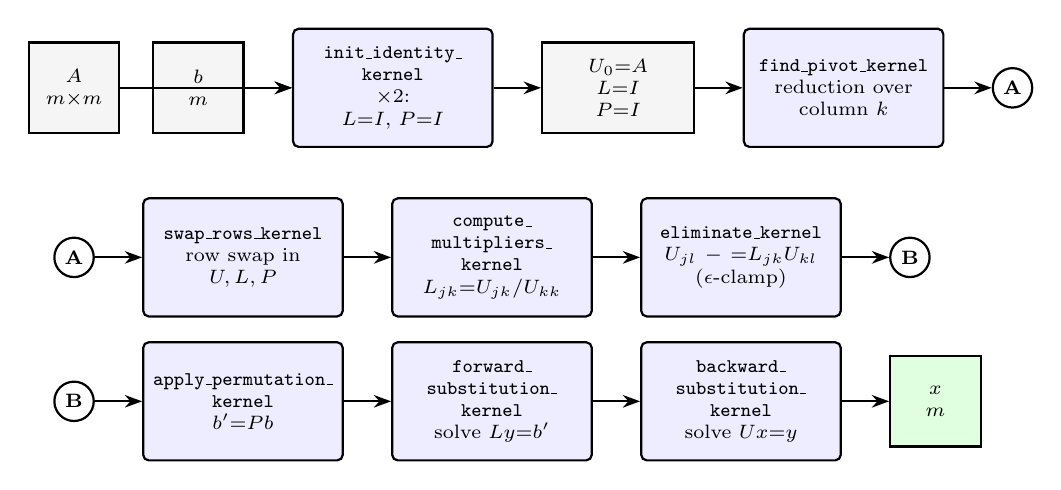
\begin{tikzpicture}[node distance=5mm and 6mm]
  % Row 1
  \node[matbox] (A) {$A$\\$m{\times}m$};
  \node[matbox, right=4mm of A] (b) {$b$\\$m$};
  \node[kernbox, right=of b] (init) {\texttt{init\_identity\_\allowbreak kernel}\\$\times 2$:\\$L{=}I$, $P{=}I$};
  \node[matbox, right=of init, minimum width=1.9cm, text width=1.7cm] (state0) {$U_0{=}A$\\$L{=}I$\\$P{=}I$};
  \node[kernbox, right=of state0] (pivot) {\texttt{find\_pivot\_\allowbreak kernel}\\reduction over\\column $k$};
  \node[contnode, right=6mm of pivot] (contA) {A};

  \draw[flowarrow] (A) -- (init);
  \draw[flowarrow] (b) -- (init);
  \draw[flowarrow] (init) -- (state0);
  \draw[flowarrow] (state0) -- (pivot);
  \draw[flowarrow] (pivot) -- (contA);

  % Row 2
  \node[contnode, below=13mm of A] (contA2) {A};
  \node[kernbox, right=6mm of contA2] (swap) {\texttt{swap\_rows\_\allowbreak kernel}\\row swap in\\$U,L,P$};
  \node[kernbox, right=of swap] (mult) {\texttt{compute\_\allowbreak multipliers\_\allowbreak kernel}\\$L_{jk}{=}U_{jk}/U_{kk}$};
  \node[kernbox, right=of mult] (elim) {\texttt{eliminate\_\allowbreak kernel}\\$U_{jl}\mathrel{-}{=}L_{jk}U_{kl}$\\($\epsilon$-clamp)};
  \node[contnode, right=6mm of elim] (contB) {B};

  \draw[flowarrow] (contA2) -- (swap);
  \draw[flowarrow] (swap) -- (mult);
  \draw[flowarrow] (mult) -- (elim);
  \draw[flowarrow] (elim) -- (contB);

  % Row 3
  \node[contnode, below=13mm of contA2] (contB2) {B};
  \node[kernbox, right=6mm of contB2] (perm) {\texttt{apply\_\allowbreak permutation\_\allowbreak kernel}\\$b'{=}Pb$};
  \node[kernbox, right=of perm] (fwd) {\texttt{forward\_\allowbreak substitution\_\allowbreak kernel}\\solve $Ly{=}b'$};
  \node[kernbox, right=of fwd] (bwd) {\texttt{backward\_\allowbreak substitution\_\allowbreak kernel}\\solve $Ux{=}y$};
  \node[outbox, right=of bwd] (x) {$x$\\$m$};

  \draw[flowarrow] (contB2) -- (perm);
  \draw[flowarrow] (perm) -- (fwd);
  \draw[flowarrow] (fwd) -- (bwd);
  \draw[flowarrow] (bwd) -- (x);
\end{tikzpicture}
\end{center}

\noindent Row~1's \texttt{find\_pivot\_kernel} through Row~2's
\texttt{eliminate\_kernel} --- the four boxes spanning
\textcircled{\scriptsize A} to \textcircled{\scriptsize B} --- are one pivot
step; the whole group repeats once per $k = 0, \dots, m{-}2$ ($m{-}1$ times
total, $m{-}1{=}19$ for the $20\times20$ matrices used here) before
continuing on to \texttt{apply\_permutation\_kernel}. The final three
kernels (Row~3) run once each, after the elimination loop completes.

\section{Stage 1: Exp-Binade Histogram Gathering}
\label{sec:binade}

\subsection{Configuration}

\texttt{bin\_spec.json} (generated by \texttt{gen\_bin\_spec.py}) configures
nixnan's \texttt{BIN\_SPEC\_FILE} binade-monitoring feature:

\begin{lstlisting}
{
    "count": 128,
    "doublings": 7,
    "max_reports": 0,
    "f16": [],
    "bf16": [],
    "f32": [],
    "f64": [[-1022, -1019], [-1018, -1015], ..., [1022, 1023]]
}
\end{lstlisting}

\begin{itemize}
  \item \textbf{All precisions present}: \texttt{lu\_solve\_gpu.cu} computes
    only in \texttt{double}, so \texttt{f64} is the only format populated
    with exponent bins; \texttt{f16}/\texttt{bf16}/\texttt{f32} are left
    empty, which is valid per nixnan's schema and correctly reflects that
    those formats are not present in the solver's source-level arithmetic
    (see Section~\ref{sec:fp32-artifact} for a caveat about what nixnan
    itself classifies at the SASS level).
  \item \textbf{Histogram bucket size 4}: the \texttt{f64} array tiles the
    full valid double exponent range $[-1022, 1023]$ (normal exponents
    only; the reserved subnormal/inf/NaN exponent codes are excluded) into
    512 buckets of width 4.
  \item \textbf{Report threshold \texttt{count: 128}}: an initial attempt
    with \texttt{count: 1} produced roughly 13{,}700 threshold-report lines
    for a single run, because nixnan reports on \emph{every} occurrence past
    the first once \texttt{count} is 1 (see the report condition in
    Section~\ref{sec:doublings}). \texttt{128} was chosen to match nixnan's
    own convention (its auto-generated template, and the
    \texttt{SC26-expts/rd\_nixnan} example, both default to this order of
    magnitude) and produces a much more legible 99--63 reports per run here.
\end{itemize}

\subsection{Results}

\begin{table}[h]
\centering
\begin{tabular}{lrrr}
\toprule
& \texttt{matrix.csv} & \texttt{bad\_matrix.csv} \\
\midrule
Residual $\lVert Ax-b\rVert_2$ (uninstrumented) & $9.68\times10^{-16}$ & \texttt{nan} \\
Binade-threshold reports & 99 & 63 \\
FP64 NaN (repeats) & 0 (0) & 316 (2171) \\
FP64 Infinity (repeats) & 0 (0) & 4 (0) \\
FP64 Division-by-zero (repeats) & 0 (0) & 4 (4) \\
\bottomrule
\end{tabular}
\caption{Stage 1 results, from \texttt{logs/baseline/*.log} and
\texttt{logs/histogram/*.log}.}
\label{tab:stage1}
\end{table}

This reproduces the CPU tutorial's central finding on the GPU: the
well-conditioned matrix produces a clean solution and no exceptions of any
kind, while the ill-conditioned matrix triggers exactly the failure the
tutorial is built around (a near-zero pivot leading to division-by-zero,
then NaN propagation through the whole solve).

\subsection{An FP32 Artifact of Binary Instrumentation}
\label{sec:fp32-artifact}

Despite the source computing exclusively in \texttt{double}, the final
report for \texttt{bad\_matrix.csv} also shows 6 FP32 NaN detections (93
repeats). Inspecting the flagged SASS instructions
(\texttt{TOOL\_VERBOSE=1}, \texttt{PRINT\_ILL\_INSTR=1}) shows the pattern
\texttt{FFMA R8, RZ, R5, R3} in \texttt{compute\_multipliers\_kernel} and
\texttt{backward\_substitution\_kernel}. This is \texttt{ptxas}'s
``multiply-by-the-zero-register'' idiom for a register move
($0 \times R5 + R3 = R3$), used here to shuffle the 32-bit halves of a
64-bit double across the register file rather than to perform a genuine
32-bit floating-point computation. Because nixnan instruments at the SASS
opcode level, it correctly classifies \texttt{FFMA} as an \texttt{f32}
instruction and correctly notices that the multiplicand \texttt{R5} happens
to hold a 32-bit sub-word bit pattern that decodes as NaN -- but that
32-bit word is a half of a double, never interpreted as an \texttt{f32}
value by the program. This is a known class of false positive for
binary-level FP exception detectors and is worth keeping in mind when
reading ``per-format'' exception counts: a nonzero count in a format the
source code never uses does not necessarily mean that format's arithmetic
ran.

\section{Stage 2: Exponential \texttt{SAMPLING} Sweep}
\label{sec:sampling}

\subsection{Requested Schedule}

The requested instrumentation-sampling schedule was: \texttt{SAMPLING=1}
for 16 runs (``snaps''), then \texttt{2} for 16, then \texttt{4} for 16,
then \texttt{8} for 16, then reset back to \texttt{1}.

nixnan reads \texttt{SAMPLING} once at process start
(\texttt{GET\_VAR\_INT(sampling, "SAMPLING", ...)} in \texttt{src/nixnan.cu})
and there is no supported way to change it mid-run. The schedule is
therefore implemented in \texttt{run\_nixnan\_experiment.sh} as 64 separate
whole-program launches of \texttt{lu\_solve\_gpu bad\_matrix.csv} (one
``snap'' = one process), storing each run's nixnan log and stdout under
\texttt{logs/sampling/cycle\_01/sampling\_\{1,2,4,8\}/snap\_\{01..16\}}.
Since the solver is deterministic (fixed CSV input, no randomness), the 16
snaps at a fixed level are expected -- and observed -- to be byte-identical;
the stored logs faithfully record the \emph{schedule}, not run-to-run
variation.

\subsection{Finding: \texttt{SAMPLING} Has No Observable Effect}
\label{sec:sampling-bug}

\texttt{bad\_matrix.csv}'s elimination kernels (Table~\ref{tab:kernels}) are
each launched $\sim$19 times, once per pivot step, so
$\texttt{SAMPLING}\in\{1,2,4,8\}$ should visibly change how many of those
repeat invocations get instrumented. It does not: \texttt{snap\_01.log} for
\texttt{SAMPLING=1} and for \texttt{SAMPLING=8} are byte-identical
(\texttt{diff} produces no output), as are all 16 snaps within any single
level (one MD5 across all 16 files).

Reading \texttt{src/nixnan.cu} explains why. The sampling-skip check lives
in \texttt{should\_instrument()}:

\begin{lstlisting}[language=C++]
bool should_instrument(CUcontext ctx, CUfunction f) {
  std::string func_name = nvbit_get_func_name(ctx, f);   // full signature
  ...
  if (sampling != 0 && analyzed_kernels.count(func_name)) {
    if (analyzed_kernels[func_name] % sampling != 0) {
      ++analyzed_kernels[func_name];
      enable_instr = false;
    }
  }
  return enable_instr;
}
\end{lstlisting}

\noindent while the counter it reads, \texttt{analyzed\_kernels}, is
incremented in the CUDA-launch callback under a \emph{different} key:

\begin{lstlisting}[language=C++]
std::string kernel_name = nvbit_get_func_name(ctx, p->f);
std::string short_name = cut_kernel_name(kernel_name);   // truncated name
...
if (enable_instr) {
  int count = analyzed_kernels[short_name]++;            // <-- keyed on short_name
  ...
  ++analyzed_kernels[short_name];
}
\end{lstlisting}

\noindent where \texttt{cut\_kernel\_name} (\texttt{src/common.cuh})
truncates at the first \texttt{<} or \texttt{(}:

\begin{lstlisting}[language=C++]
inline std::string cut_kernel_name(const std::string& kernel_name) {
  size_t pos = kernel_name.find_first_of("<(");
  if (pos != std::string::npos) return kernel_name.substr(0, pos);
  return kernel_name;
}
\end{lstlisting}

For a kernel such as
\texttt{eliminate\_kernel(double*, double const*, int, int)}, the two keys
are \texttt{"eliminate\_kernel(double*, double const*, int, int)"} (full
signature, used in the lookup) versus \texttt{"eliminate\_kernel"}
(truncated, used for the increment). These never match for any kernel with
a non-empty parameter list -- i.e.\ essentially every real CUDA kernel --
so \texttt{analyzed\_kernels.count(func\_name)} is always \texttt{0} inside
\texttt{should\_instrument()}, the skip branch never executes, and every
invocation is instrumented irrespective of \texttt{SAMPLING}. This appears
to be a genuine bug in nixnan's \texttt{SAMPLING} feature, independent of
this experiment, and worth fixing upstream. The 64 stored logs remain a
faithful record of the requested schedule and harness, but currently
demonstrate no sampling-induced difference in coverage.

\section{A Second Documentation/Implementation Gap: \texttt{doublings}}
\label{sec:doublings}

nixnan's documentation (\texttt{README.md}, \texttt{Tutorial.md}) describes
a \texttt{doublings} field for \texttt{BIN\_SPEC\_FILE} that adaptively
scales the report threshold ($256\to512\to1024\to\cdots\to$ reset). As of
this checkout, \texttt{src/fp-histogram.cu} never reads that key. The only
threshold logic is in \texttt{record()} (\texttt{src/fp-fun.cu}):

\begin{lstlisting}[language=C++]
unsigned long long int prev = bin.increment();
if (prev % count == 0 && prev != 0) {
    // ... send report ...
}
\end{lstlisting}

which reports every time the running count is a positive multiple of the
\emph{static} \texttt{count} threshold -- with no reference to a doubling
schedule anywhere in \texttt{src/}. \texttt{bin\_spec.json} still sets
\texttt{doublings} for schema/forward compatibility, but it is currently a
no-op. This is why Stage 2's exponential schedule was implemented at the
shell-script level (Section~\ref{sec:sampling}) rather than relying on
\texttt{BIN\_SPEC\_FILE}.

\section{Tensor-Core Adaptation: \texttt{lu\_solve\_gpu\_tc.cu}}
\label{sec:tc}

\texttt{lu\_solve\_gpu.cu} updates the trailing matrix with a rank-1
update per pivot (\texttt{eliminate\_kernel}), which is a scalar FP64
operation and cannot use tensor cores. To obtain an instruction stream that
contains \texttt{HMMA}, the factorization was restructured as a standard
\emph{blocked, right-looking} LU with block size $NB=16$ (equal to the WMMA tile
edge). The rank-1 updates of a block of 16 pivots are accumulated into one
matrix--matrix product, and that product is computed on the tensor cores.
Everything else (pivoting, the panel, the triangular solve,
the substitutions, the residual) stays in FP64; this is a mixed-precision LU
without iterative refinement. The RTX~3090 (sm\_86) has no FP64 tensor cores,
so the WMMA inputs are FP16 or BF16.

\subsection{What changes in the algorithm}

\begin{center}
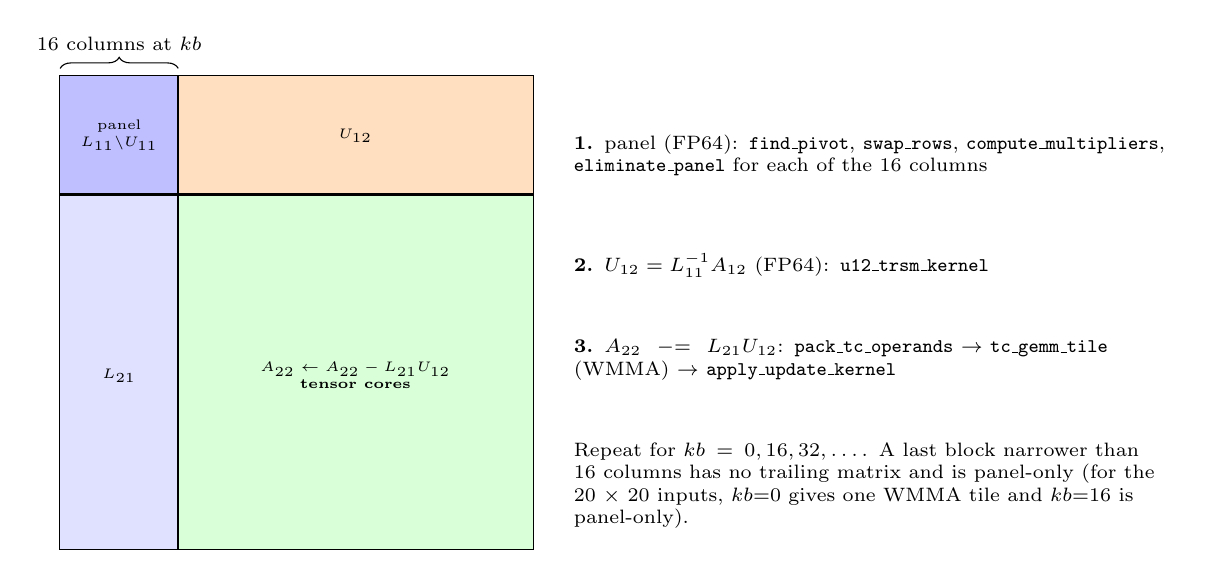
\begin{tikzpicture}[x=1cm,y=1cm]
  \def\w{6.0}
  \draw[thick] (0,0) rectangle (\w,\w);
  \fill[blue!25] (0,\w-1.5) rectangle (1.5,\w);
  \fill[blue!12] (0,0) rectangle (1.5,\w-1.5);
  \fill[orange!25] (1.5,\w-1.5) rectangle (\w,\w);
  \fill[green!15] (1.5,0) rectangle (\w,\w-1.5);
  \draw[thick] (1.5,0) -- (1.5,\w);
  \draw[thick] (0,\w-1.5) -- (\w,\w-1.5);
  \node[font=\tiny,align=center] at (0.75,\w-0.75) {panel\\$L_{11}\backslash U_{11}$};
  \node[font=\tiny,align=center] at (0.75,2.2) {$L_{21}$};
  \node[font=\tiny,align=center] at (3.75,\w-0.75) {$U_{12}$};
  \node[font=\tiny,align=center] at (3.75,2.2) {$A_{22}\leftarrow A_{22}-L_{21}U_{12}$\\\textbf{tensor cores}};
  \draw[decorate,decoration={brace,amplitude=4pt}] (0,\w+0.1) -- (1.5,\w+0.1)
        node[midway,above=3pt,font=\scriptsize]{16 columns at $kb$};
  \node[font=\scriptsize,anchor=west,align=left,text width=7.6cm] at (6.4,5.0)
     {\textbf{1.} panel (FP64): \texttt{find\_pivot}, \texttt{swap\_rows}, \texttt{compute\_multipliers}, \texttt{eliminate\_panel} for each of the 16 columns};
  \node[font=\scriptsize,anchor=west,align=left,text width=7.6cm] at (6.4,3.6)
     {\textbf{2.} $U_{12}=L_{11}^{-1}A_{12}$ (FP64): \texttt{u12\_trsm\_kernel}};
  \node[font=\scriptsize,anchor=west,align=left,text width=7.6cm] at (6.4,2.4)
     {\textbf{3.} $A_{22}\mathrel{-}=L_{21}U_{12}$: \texttt{pack\_tc\_operands} $\to$ \texttt{tc\_gemm\_tile} (WMMA) $\to$ \texttt{apply\_update\_kernel}};
  \node[font=\scriptsize,anchor=west,align=left,text width=7.6cm] at (6.4,0.8)
     {Repeat for $kb=0,16,32,\dots$. A last block narrower than 16 columns has no trailing matrix and is panel-only (for the $20\times20$ inputs, $kb{=}0$ gives one WMMA tile and $kb{=}16$ is panel-only).};
\end{tikzpicture}
\end{center}

Row swaps still act on the full row of $U$ (and on $P$, and on the already
computed columns of $L$), so the right-hand blocks $A_{12}$ and $A_{22}$ stay
consistent with the pivoting done in the panel. The $\epsilon$-clamp of the
original (\texttt{|val| < 10*DBL\_EPSILON} $\to 0$) is kept in both the panel
elimination and the trailing update.

\subsection{Kernel pipeline for one block step}

\begin{center}
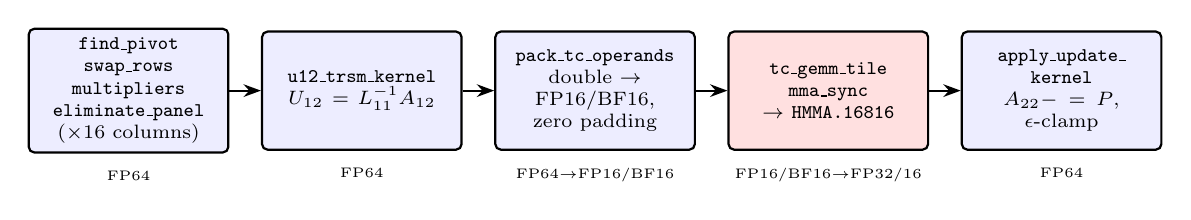
\begin{tikzpicture}[node distance=4mm and 4mm,
    k64/.style={kernbox, fill=blue!7, text width=2.3cm, minimum width=2.5cm, minimum height=1.5cm},
    ktc/.style={kernbox, fill=red!12, text width=2.3cm, minimum width=2.5cm, minimum height=1.5cm}]
  \node[k64] (piv) {\texttt{find\_pivot} \texttt{swap\_rows} \texttt{multipliers} \texttt{eliminate\_\allowbreak panel}\\($\times16$ columns)};
  \node[k64, right=of piv] (trsm) {\texttt{u12\_trsm\_\allowbreak kernel}\\$U_{12}=L_{11}^{-1}A_{12}$};
  \node[k64, right=of trsm] (pack) {\texttt{pack\_tc\_\allowbreak operands}\\double $\to$ FP16/BF16, zero padding};
  \node[ktc, right=of pack] (gemm) {\texttt{tc\_gemm\_tile}\\\texttt{mma\_sync}\\$\to$ \texttt{HMMA.16816}};
  \node[k64, right=of gemm] (upd) {\texttt{apply\_update\_\allowbreak kernel}\\$A_{22}-=P$,\\$\epsilon$-clamp};
  \draw[flowarrow] (piv) -- (trsm);
  \draw[flowarrow] (trsm) -- (pack);
  \draw[flowarrow] (pack) -- (gemm);
  \draw[flowarrow] (gemm) -- (upd);
  \node[font=\tiny, below=1mm of piv] {FP64};
  \node[font=\tiny, below=1mm of trsm] {FP64};
  \node[font=\tiny, below=1mm of pack] {FP64$\to$FP16/BF16};
  \node[font=\tiny, below=1mm of gemm] {FP16/BF16$\to$FP32/16};
  \node[font=\tiny, below=1mm of upd] {FP64};
\end{tikzpicture}
\end{center}

\noindent Blue boxes are FP64; the red box is the only tensor-core kernel. The
\texttt{pack} and \texttt{update} kernels bracket it and perform the
precision conversions: they are where values enter and leave reduced
precision.

\subsection{Data path of the trailing update}

\begin{center}
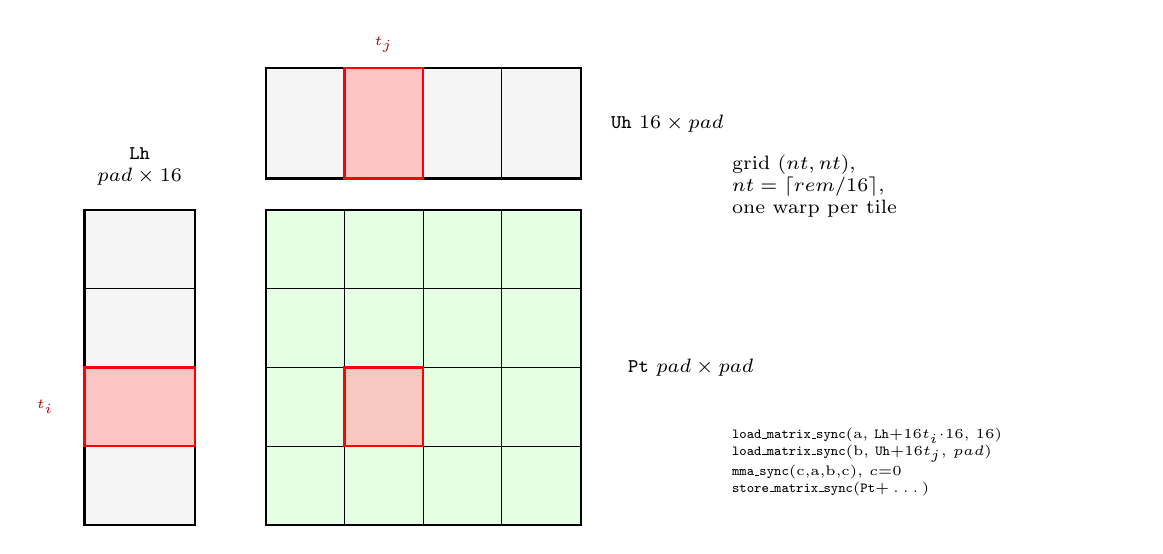
\begin{tikzpicture}[x=1cm,y=1cm]
  \draw[thick,fill=gray!8] (0,0) rectangle (1.4,4);
  \foreach \y in {1,2,3} {\draw (0,\y) -- (1.4,\y);}
  \node[font=\scriptsize,align=center] at (0.7,4.55) {\texttt{Lh}\\$pad\times16$};
  \draw[thick,fill=gray!8] (2.3,4.4) rectangle (6.3,5.8);
  \foreach \x in {3.3,4.3,5.3} {\draw (\x,4.4) -- (\x,5.8);}
  \node[font=\scriptsize] at (7.4,5.1) {\texttt{Uh}\ $16\times pad$};
  \draw[thick,fill=green!10] (2.3,0) rectangle (6.3,4.0);
  \foreach \x in {3.3,4.3,5.3} {\draw (\x,0) -- (\x,4.0);}
  \foreach \y in {1,2,3} {\draw (2.3,\y) -- (6.3,\y);}
  \node[font=\scriptsize] at (7.7,2.0) {\texttt{Pt}\ $pad\times pad$};
  \fill[red!30,opacity=.7] (3.3,1) rectangle (4.3,2);
  \draw[red,thick] (3.3,1) rectangle (4.3,2);
  \fill[red!30,opacity=.7] (0,1) rectangle (1.4,2);
  \draw[red,thick] (0,1) rectangle (1.4,2);
  \fill[red!30,opacity=.7] (3.3,4.4) rectangle (4.3,5.8);
  \draw[red,thick] (3.3,4.4) rectangle (4.3,5.8);
  \node[font=\tiny,red!70!black] at (-0.5,1.5) {$t_i$};
  \node[font=\tiny,red!70!black] at (3.8,6.1) {$t_j$};
  \node[font=\scriptsize,align=left,anchor=west] at (8.1,4.3) {grid $(nt,nt)$,\\$nt=\lceil rem/16\rceil$,\\one warp per tile};
  \node[font=\tiny,align=left,anchor=west,text width=5cm] at (8.1,0.8) {\texttt{load\_matrix\_sync}(a, \texttt{Lh}$+16t_i{\cdot}16$, 16)\\ \texttt{load\_matrix\_sync}(b, \texttt{Uh}$+16t_j$, $pad$)\\ \texttt{mma\_sync}(c,a,b,c), $c{=}0$\\ \texttt{store\_matrix\_sync}(\texttt{Pt}$+\dots$)};
\end{tikzpicture}
\end{center}

\noindent Padding rows and columns (beyond $m$) are exact zeros, so a tile
that straddles the matrix edge computes the right values. The accumulator
starts at zero (\texttt{fill\_fragment}); this is why the compiled
\texttt{HMMA} has \texttt{RZ} as its C operand in the first instruction.
\texttt{apply\_update\_kernel} then reads \texttt{Pt}, widens to double, and
subtracts from $A_{22}$.

\subsection{From WMMA to SASS}

\begin{center}
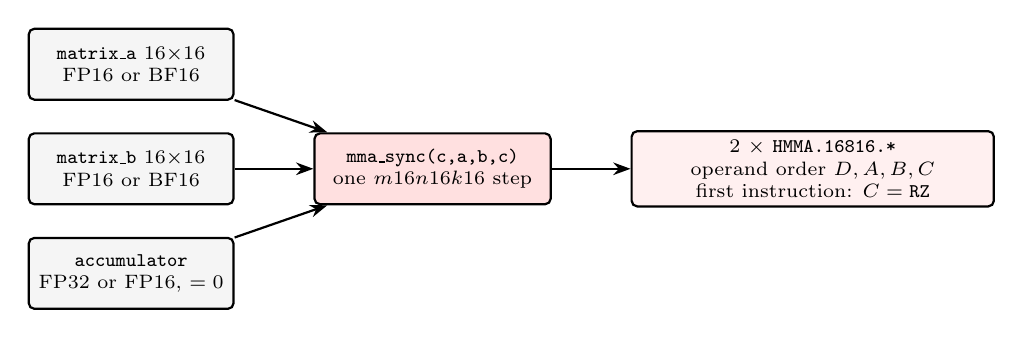
\begin{tikzpicture}[node distance=4mm and 8mm,
    fr/.style={draw,thick,rounded corners=2pt,font=\scriptsize,align=center,minimum height=0.9cm,minimum width=2.6cm,fill=gray!8}]
  \node[fr] (a) {\texttt{matrix\_a} $16{\times}16$\\FP16 or BF16};
  \node[fr, below=of a] (b) {\texttt{matrix\_b} $16{\times}16$\\FP16 or BF16};
  \node[fr, below=of b] (c) {\texttt{accumulator}\\FP32 or FP16, $=0$};
  \node[fr, right=10mm of b, fill=red!12, minimum width=3.0cm] (mma) {\texttt{mma\_sync(c,a,b,c)}\\one $m16n16k16$ step};
  \node[fr, right=10mm of mma, fill=red!6, minimum width=4.6cm] (s)
     {2 $\times$ \texttt{HMMA.16816.*}\\operand order $D,A,B,C$\\first instruction: $C=\texttt{RZ}$};
  \draw[flowarrow] (a) -- (mma);
  \draw[flowarrow] (b) -- (mma);
  \draw[flowarrow] (c) -- (mma);
  \draw[flowarrow] (mma) -- (s);
\end{tikzpicture}
\end{center}

\begin{center}
\small
\begin{tabular}{llll}
\toprule
Mode & WMMA types & SASS & Count in binary\\
\midrule
\texttt{fp16acc32} & \texttt{half}$\times$\texttt{half}$\to$\texttt{float} & \texttt{HMMA.16816.F32} & 2\\
\texttt{fp16acc16} & \texttt{half}$\times$\texttt{half}$\to$\texttt{half} & \texttt{HMMA.16816.F16} & 2\\
\texttt{bf16acc32} & \texttt{bf16}$\times$\texttt{bf16}$\to$\texttt{float} & \texttt{HMMA.16816.F32.BF16} & 2\\
\bottomrule
\end{tabular}
\end{center}

\noindent The count (checked with \texttt{cuobjdump -sass}) is 2 per mode:
one \texttt{mma\_sync} lowers to two \texttt{HMMA.16816} instructions. That
they cover the two 8-column halves of the $16\times16$ output is the
standard decomposition and was not separately verified.

\subsection{Where reduced-precision exceptions can arise}

\begin{center}
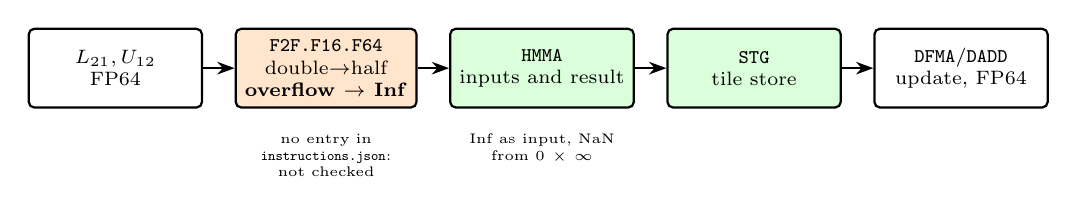
\begin{tikzpicture}[node distance=3mm and 4mm,
   st/.style={draw,thick,rounded corners=2pt,font=\scriptsize,align=center,minimum height=1.0cm,minimum width=2.2cm},
   seen/.style={st,fill=green!14}, unseen/.style={st,fill=orange!20}]
  \node[st] (d) {$L_{21}, U_{12}$\\FP64};
  \node[unseen, right=of d] (f2f) {\texttt{F2F.F16.F64}\\double$\to$half\\\textbf{overflow $\to$ Inf}};
  \node[seen, right=of f2f] (h) {\texttt{HMMA}\\inputs and result};
  \node[seen, right=of h] (stg) {\texttt{STG}\\tile store};
  \node[st, right=of stg] (fp64) {\texttt{DFMA}/\texttt{DADD}\\update, FP64};
  \draw[flowarrow] (d) -- (f2f);
  \draw[flowarrow] (f2f) -- (h);
  \draw[flowarrow] (h) -- (stg);
  \draw[flowarrow] (stg) -- (fp64);
  \node[font=\tiny, below=2mm of f2f, text width=2.4cm, align=center] {no entry in \texttt{instructions.json}: not checked};
  \node[font=\tiny, below=2mm of h, text width=2.4cm, align=center] {Inf as input, NaN from $0\times\infty$};
\end{tikzpicture}
\end{center}

\noindent Green boxes are instructions nixnan checks in this build; orange is
an instruction it does not. The findings below match this picture.

\section{Findings from the Tensor-Core Version}
\label{sec:tcfindings}

All runs: RTX~3090, CUDA~12.4, nixnan branch \texttt{print\_histo\_instrn}
(commit \texttt{ce35185}), launched with \texttt{env -u LD\_LIBRARY\_PATH}
(with the stale \texttt{LD\_LIBRARY\_PATH} nixnan printed only its banner;
the individual entry causing this was not isolated). Logs are in
\texttt{logs/tc/}.

\subsection{Numerical behaviour}

\begin{center}
\small
\begin{tabular}{lcccc}
\toprule
Input & \texttt{fp16acc32} & \texttt{fp16acc16} & \texttt{bf16acc32} & FP64 original\\
\midrule
\texttt{matrix.csv} residual & $1.1\!\times\!10^{-4}$ & $2.0\!\times\!10^{-4}$ & $4.4\!\times\!10^{-4}$ & $9.7\!\times\!10^{-16}$\\
\texttt{bad\_matrix.csv} & NaN & NaN & NaN & NaN\\
\texttt{rand:64:100000} & NaN & NaN & 0.17 & --\\
\bottomrule
\end{tabular}
\end{center}

\begin{itemize}
  \item On the well-conditioned input the tensor-core product costs about
    twelve orders of magnitude of residual (reduced-precision $L_{21}U_{12}$,
    no refinement). BF16 is the least accurate and the FP16 accumulator is
    slightly worse than the FP32 one.
  \item The ill-conditioned input fails exactly as in the FP64 code, so the
    failure originates in the FP64 near-zero pivot, not in the tensor cores.
  \item Residuals grow with $n$ (\texttt{rand:256:1}: 0.75 FP16, 5.4 BF16).
    The random matrices' conditioning was not examined, so this is reported
    as observed, not explained.
  \item With entries scaled by $10^5$, FP16 conversion overflows (65504 max)
    and the solve returns NaN, whereas BF16 (FP32-like range) completes.
\end{itemize}

\subsection{What nixnan reports}

\begin{itemize}
  \item \textbf{No exceptions} for \texttt{matrix.csv} (all three modes) and
    for \texttt{rand:64:100000} in \texttt{bf16acc32}.
  \item \textbf{FP16 modes with overflow} (\texttt{rand:64:100000}, 435 error
    lines in each log): the first report is \texttt{[infinity]} in
    \emph{operand 2} (B, the $U_{12}$ fragment, type f16) of
    \texttt{HMMA.16816.F32} (or \texttt{.F16}). NaN follows in operand 0 (the
    HMMA result), then on the \texttt{STG} that stores the tile, then as FP64
    NaN/Inf in \texttt{DFMA}/\texttt{DADD} of the update. The
    \texttt{fp16acc32} summary shows FP32 NaN 14 (376 repeats), Infinity 4
    (6), $-$Infinity 4 (6) and FP64 NaN 406 (18642 repeats), Infinity 19
    (70), $-$Infinity 12 (56).
  \item \textbf{Why NaN so quickly:} the padding of \texttt{Lh}/\texttt{Uh} is
    exact zeros and the tensor core computes every product, so
    $0\times\infty=\mathrm{NaN}$ spreads the Inf across its tile row and
    column (the same effect seen in the 2D reaction--diffusion kernel).
  \item \textbf{The origin of the Inf is not reported.} It is created by
    \texttt{F2F.F16.F64} (double$\to$half in \texttt{pack\_tc\_operands}),
    which has no entry in \texttt{instructions.json}, so nixnan sees it only
    as an input of the next HMMA. The first Inf reported is in operand 2
    ($U_{12}$), not operand 1 ($L_{21}$, bounded by 1 in magnitude under
    partial pivoting).
  \item \textbf{Source lines:} \texttt{LINE\_INFO=1} resolved no source
    location for these kernels (no match for \texttt{lu\_solve\_\allowbreak gpu\_tc.cu}
    in any log), although the binary is built with \texttt{-lineinfo}.
\end{itemize}

\subsection{Limits of these results}

\begin{itemize}
  \item Only the $20\times20$ inputs and \texttt{rand:} matrices were run; the
    $20\times20$ case exercises a single WMMA tile.
  \item No iterative refinement: the residuals are those of a single
    mixed-precision factorization.
  \item The per-HMMA register walkthrough (\texttt{TOOL\_VERBOSE=1}) was done
    for the reaction--diffusion kernel, not repeated for this program.
\end{itemize}

\section{Conclusions}

\begin{enumerate}
  \item The GPU port of the tutorial's LU solver reproduces the CPU
    behavior exactly at the level that matters for the tutorial's purpose:
    clean convergence on a well-conditioned system, and NaN/Inf/Div-by-zero
    on an ill-conditioned one, both correctly detected and attributed by
    nixnan's exception instrumentation and its exp-binade histogram
    feature.
  \item Two tool-level gaps were found and documented with code-level
    evidence: \texttt{SAMPLING} does not filter any instrumentation in this
    build (Section~\ref{sec:sampling-bug}), and \texttt{BIN\_SPEC\_FILE}'s
    \texttt{doublings} field is unimplemented (Section~\ref{sec:doublings}).
    Neither was fixed here (out of scope for this experiment), but both are
    concrete, reproducible findings for the nixnan maintainers.
  \item Binary-level FP exception detection can misattribute a compiler
    register-move idiom as a genuine narrow-format computation
    (Section~\ref{sec:fp32-artifact}); per-format counts should be read
    alongside the source's actual precision usage, not in isolation.
  \item A tensor-core variant (blocked LU, WMMA trailing update;
    Sections~\ref{sec:tc}--\ref{sec:tcfindings}) shows nixnan flagging
    \texttt{HMMA.16816.\{F16,F32\}} inputs and results when FP16
    conversion overflows, but not the \texttt{F2F.F16.F64} conversion that
    creates the Inf.
\end{enumerate}

\section*{Reproduction}

\begin{lstlisting}
cd ~/repos/nixnan/SC26-expts/lu_solve_gpu
./run_nixnan_experiment.sh
\end{lstlisting}

\noindent Tensor-core version: \texttt{make lu\_solve\_gpu\_tc}, then \texttt{env -u LD\_LIBRARY\_PATH LD\_PRELOAD=../../nixnan.so ./lu\_solve\_gpu\_tc rand:64:100000 fp16acc32}.

\noindent Requires a built \texttt{../../nixnan.so} (\texttt{cd ../.. \&\& make}).
See \texttt{README.md} in this directory for file-by-file documentation and
override variables (\texttt{NIXNAN\_SO}, \texttt{CYCLES},
\texttt{SAMPLING\_MATRIX}).

\end{document}
